\documentclass{ctrlo-int-toc}

\setdate{30th June 2016}

\settitle{linkspace user guide}

\setname{Linkspace User Guide}

\usepackage{supertabular}
\usepackage{comment}
% \excludecomment{admin}
\includecomment{admin}

\begin{document}

\clearpage\section{Quick start guide for Linkspace users}
\label{sec:quickstart}
Linkspace has been designed to make it easy for teams, departments and organisations to share and update information across multiple locations.

As a general Linkspace user, once you have logged in, almost everything you need can be found under the \textbf{Data} tab. Exactly what you can do in the system will depend on the permissions you have been given by the system administrator though. You may only be able to view data, or you may be able to \hyperref[subsec:addrecord]{add records} or just \hyperref[subsec:editrecord]{edit records}.

\subsection{using the power of data views}
One of the things that makes Linkspace easy to use is that it allows you to quickly see only the data you need, rather than having to contend with columns and rows of data that may be irrelevant to your team or your specific tasks. You can save sorted and filtered views of the data so that you can access them immediately when you log in.

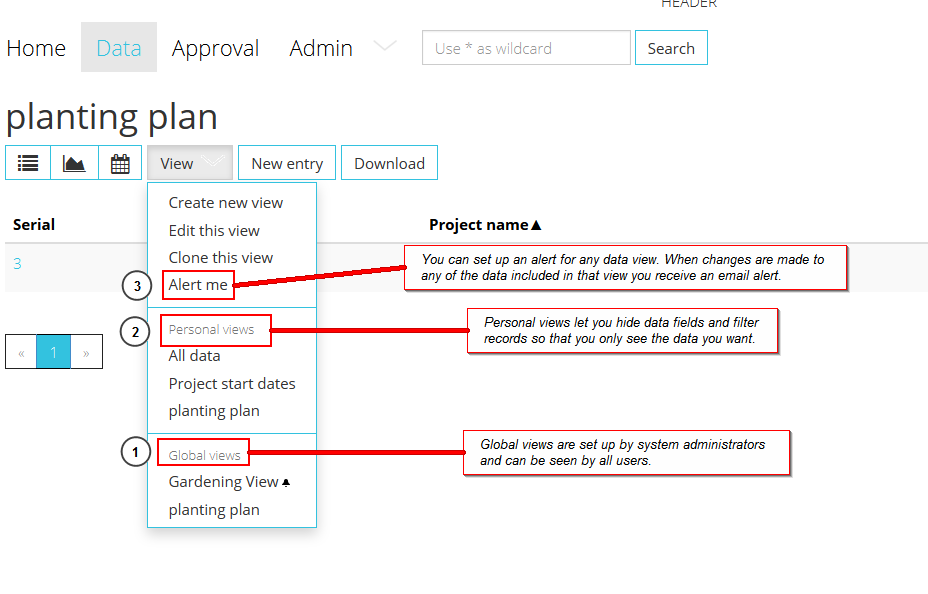
\includegraphics[width=15.921cm,height=10.188cm]{userguide-img/userguide-img001.png}


You can also set up alerts for any of your data views. Once you have set an alert on a view, you will receive a notification when any data for that view is updated, or new data is added.

Under the \textbf{Data} {\textgreater} \textbf{View} dropdown menu, you can see \hyperref[subsec:globalview]{global views}. These are views of the data that are set up by the systems administrators. You may also have the permissions to \hyperref[subsec:personalview]{set up personalised data views}, which let you set up your own views, filtering and sorting records and hiding anything you don't need.

You can also \hyperref[subsec:setalert]{set up alerts} for any of your data views. Once you have set an alert on a view, you will receive a notification when any data for that view is updated, or new data is added.

\clearpage\section[RECORDS: Adding, editing and deleting records]{RECORDS: Adding, editing and deleting records}
\subsection[add a new record]{add a new record}
\label{subsec:addrecord}
\begin{enumerate}
\item Click the \textbf{Data} tab in the top navigation 
\item Click the \textbf{New record} button. If you do not have this button then you do not have permission to add new records.
\item Fill in the fields and click \textbf{Save}.
\end{enumerate}
\begin{notebox}
NOTE: If your new record needs to be approved, you won't see it included in the data until someone with the correct permissions approves it. In this case, when you click on Save you should see a message confirming that your record has been submitted for approval. Otherwise you should see a message saying that your ``Submission has been completed successfully.''
\end{notebox}

\subsection[edit a record]{edit a record}
\label{subsec:editrecord}
\begin{enumerate}
\item Click the \textbf{Data} tab in the top navigation.
\item If you can't see the record you want to edit, click on the \textbf{View} dropdown and select the \hyperref[sec:views]{data view} that will show you the record you need.
\item Alternatively, use the \textbf{Search} box at the top of the page to find your record.
\item Click \textbf{Edit} next to the number listed in the \textbf{ID} column of the record you want to edit.
\item If you do not have this button then you do not have permission to edit records.
\item Make any changes and click the \textbf{Save} button at the bottom of the record.
\end{enumerate}
\begin{notebox}
NOTE: If your edits need to be approved, you won't see them immediately. In this case, when you click on Save you should see a message confirming that your edits have been submitted for approval. Otherwise you should see a message saying that your ``Submission has been completed successfully.''
\end{notebox}

\subsection[delete a record]{delete a record}
\begin{enumerate}
\item Click the \textbf{Data} tab in the top navigation.
\item If you cannot see the record you want to edit, click on the \textbf{View} dropdown and select the \hyperref[sec:views]{data view} that will show you the record you need.
\item Alternatively, use the \textbf{Search} box at the top of the page to find your record.
\item Click on the number listed in the \textbf{Serial} column of the record you want to edit.
\item Open the \textbf{Action} menu and then click the \textbf{Delete} button. If you do not have this button then you do not have permission to delete records.
\item To confirm you want to delete the record, click the \textbf{Delete} button in the pop-up box that appears on your screen. 
\end{enumerate}
\subsection[view earlier versions of a record]{view earlier versions of a record}
\begin{enumerate}
\item Click the \textbf{Data} tab in the top navigation.
\item If you cannot see the record you want to edit, click on the \textbf{View} dropdown and select the \hyperref[sec:views]{data view} that will show you the record you need.
\item Alternatively, use the \textbf{Search} box at the top of the page to find your record.
\item Click on the number listed in the \textbf{ID} column of the record you want to edit.
\item Click the \textbf{Version history} dropdown below the Record ID and select the version you wish to view. \ 
\end{enumerate}
\subsection[sort your records]{sort your records}
\begin{enumerate}
\item Click on any of the \textbf{field names} (column headers in bold) to sort the records according to the data in that column. 
\item Click once to sort in ascending order, and a second time to sort in descending order.
\end{enumerate}
\begin{tipbox}[userdefinedwidth=15cm]
    \textbf{Tip:} To save time you can \hyperref[subsec:personalview]{set up a personalised data view}. This lets you customise and save the way you want your records to be sorted and displayed.
\end{tipbox}

\begin{notebox}
NOTE: When configuring the system, administrators can set the default sort by going to Admin {\textgreater} General settings
\end{notebox}

\subsection[filter your records ]{filter your records }
See: \hyperref[subsec:viewstofilter]{Use views to filter your data}

\subsection[download your data]{download your data}
If you have the permission to download data you will see a \textbf{Download} button in the row of icons at the top of any of your data views. Click the Download button, choose whether to Save or Download the file and click OK. 

\clearpage\section[VIEWS: Viewing your data]{VIEWS: Viewing your data}
\label{sec:views}
Linkspace lets you create and save different views of the data so that you can hide any data that's irrelevant to you for specific tasks and focus on what you need.

\textbf{Global views} are set up by system administrators and can be seen by all users. Any user with the appropriate permissions can also set up their own \textbf{personalised views}.

\subsection[create a global view]{create a global view}
\label{subsec:globalview}
Global views can be seen by all users. Not all users will have the permissions to create global views though.

\begin{enumerate}
\item Click the \textbf{Data} tab in the top navigation.
\item Click on the \textbf{View} dropdown and select the \textbf{Create new view} option.
\item On the Customise view page, type a name for your view in the \textbf{View name} box.
\item If you have the permission to create a global view you will see a \textbf{Global view tick box} under the View name box. Tick this box. 
\item Now tick the boxes next to the fields (columns) that you want to display in your final view. (You can click on the check box next to Field name to select or deselect all of them.)
\begin{notebox}
NOTE: If you want to filter the records (rows) shown in your view according to specific criteria you can use the filter form. See: \hyperref[subsec:viewstofilter]{Use views to filter your data}
\end{notebox}

\item To set the default order in which you want the final records to be displayed click on the \textbf{Add new sort} button. \ Select the field you want to sort by, and whether you want to display the results in ascending or descending order.
\item Finally, to create your view, click on the \textbf{Save} button at the bottom of your page. 
\end{enumerate}
\begin{tipbox}[userdefinedwidth=15cm]
    \textbf{Tip:} You can \hyperref[subsec:setalert]{set up alerts} to notify you of any updates to the records shown in a specific view.
\end{tipbox}

\subsection[create a personalised view]{create a personalised view}
\label{subsec:personalview}
Creating personalised views makes it easy for you to see only the data you want to see. It lets you hide fields that may not be relevant to you, and filter and sort according to your own criteria. Personalised views can only be seen by you, and there is no limit to how many you can create. Not all users will have the permissions to create personalised views though. 

\begin{enumerate}
\item Click the \textbf{Data} tab in the top navigation.
\item Click on the \textbf{View} dropdown and select the \textbf{Create new view} option. If you do not have this menu item then you do not have permission to create views.
\begin{notebox}
NOTE: You can also create a new personalised view by modifying an existing view. To do this select Clone this view instead of Create new view from the View dropdown. 
\end{notebox}

\item On the Customise view page, type a name for your view in the \textbf{View name} box.
\item Now tick the boxes next to the fields (columns) that you want to display in your final view. (You can click on the check box next to Field name to select all of them.)
\begin{notebox}
NOTE: If you want to filter the records (rows) shown in your view according to specific criteria you can use the filter form. See: \hyperref[subsec:viewstofilter]{Use views to filter your data}
\end{notebox}

\item To set the default order in which you want the final records to be displayed click on the \textbf{Add new sort} button. \ Select the field you want to sort by, and whether you want to display the results in descending or ascending order. 
\begin{notebox}
NOTE: You can also sort within a sort, i.e. you can sort by Country for example, and then sort by the cities within each country. You can continue to add multiple sort criteria in this way.
\end{notebox}

\item Finally, to create your view, click on the \textbf{Save} button at the bottom of your page. 
\end{enumerate}
\begin{tipbox}[userdefinedwidth=15cm]
    \textbf{Tip:} You can \hyperref[subsec:setalert]{set up alerts} to notify you of updates to the records shown in a specific view.
\end{tipbox}

\subsection[use views to filter your data ]{use views to filter your data }
\label{subsec:viewstofilter}
Filters can be used to only show records (rows) that meet specific criteria, making it easier to work with the data.

\begin{enumerate}
\item Click the \textbf{Data} tab in the top navigation.
\item To filter your records you need to create a new view. To do this, click on the \textbf{View} dropdown and select the \textbf{Create new view} option. If you do not have this menu item then you do not have permission to create views.
\item On the Customise view page, type a name for this view in the \textbf{View name} box.
\item Check the boxes of the fields that you want to be able to see in your final filtered list. (Click on the check box next to \textbf{Field name} to select or deselect all of them.)
\item Now create your filters using the \textbf{Filters} form.
\item Start by selecting the field you want the filter to apply to from the dropdown box. (Note that if you change the field you will need to re-enter your search criteria).
\item Use the next two boxes in the row to set the criteria for the filter. FOR EXAMPLE: If you only want to display projects that are in Australia, you would select Country from the list of data fields, then select equals from the second box, and then type Australia into the final value box. \newline
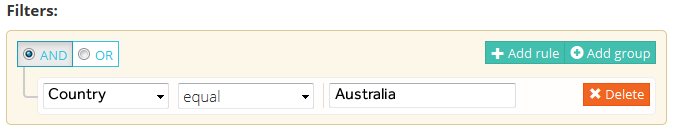
\includegraphics[width=15.921cm,height=3.069cm]{userguide-img/userguide-img002.png}
 

\begin{notebox}
NOTE
If you want to use dates in your filters use the form YYYY-MM-DD.\newline
If you want to filter by today's date, enter CURDATE in the value box. If you want to filter by your own name (i.e. the current user), enter CURUSER in the value box. 
\end{notebox}

Besides using a filter to look for an exact term or value, you can apply a number of specialized filters. These include:

\begin{flushleft}
\tablefirsthead{}
\tablehead{}
\tabletail{}
\tablelasttail{}
\begin{supertabular}{|m{3.046cm}|m{10.915cm}|}
\hline
Equal &
When you want an exact match for text or a number\\\hline
Not Equal &
When you want everything except a specific term or number.\\\hline
Less &
When you want to display only the records where the value of this field is less than a specific number, `lower' in the alphabet, or comes before a specific date. \ \\\hline
Less or Equal &
As above, but it also includes records with the value you specify. \ \\\hline
Greater  &
When you want to display only the records where the value of this field is greater than a specific number, `higher' in the alphabet or comes after a specific date. \ \\\hline
Greater or Equal &
As above, but it also includes the records with the value you specify. \ \\\hline
Begins with &
When you want to display only records that begin with a certain word or group of letters.\\\hline
\end{supertabular}
\end{flushleft}
\end{enumerate}

\subsection[apply more than one filter to a view]{apply more than one filter to a view}
\begin{enumerate}
\item You can apply several filters at the same time. For example, if you wanted to display projects that are in Australia and South Africa, you would add an OR filter, because you want to view all records where the value for Country is either South Africa or Australia. To do this select \textbf{OR} from the top of the filter box and then click the \textbf{Add rule}.\newline
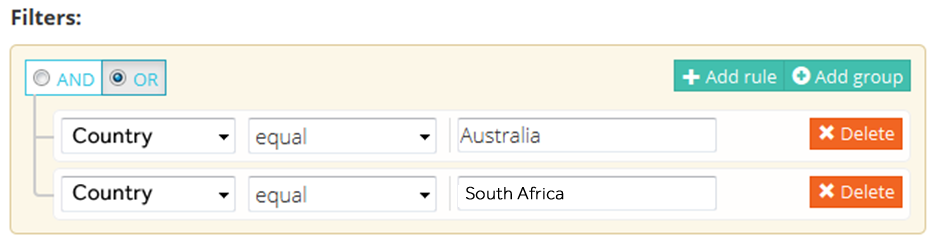
\includegraphics{userguide-img/userguide-img003.png}
 

\item You can use an AND filter if you only want to display records that meet both the criteria you set. For example, if you wanted to see all projects that were in Australia and where the project partner was ABC Corporation, you would select \textbf{AND} from the top of the filter box and then click the \textbf{Add rule}.\newline
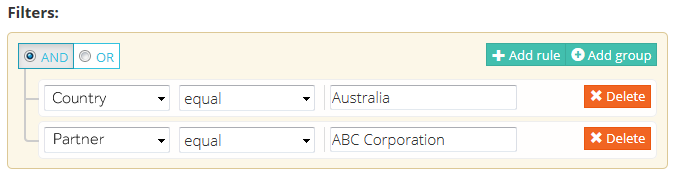
\includegraphics[width=15.667cm,height=4.055cm]{userguide-img/userguide-img004.png}
 

\item You can \textbf{group your filters} to nest different criteria. \ For example, if you wanted to see projects where the partner was ABC Corporation and that are in either Australia or Japan, you would add the two countries as a separate sub-group.

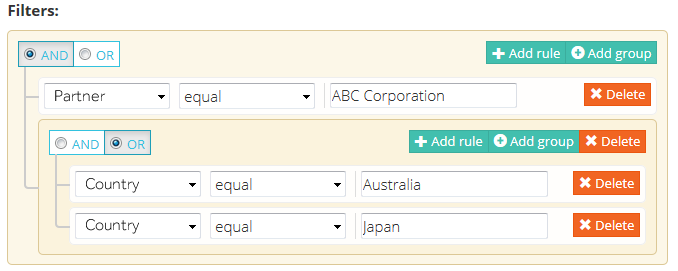
\includegraphics[width=15.693cm,height=6.272cm]{userguide-img/userguide-img005.png}
 

\item If you want to use dates in your filters you need to use the form \textbf{yyyy-mm-dd}. To create a view that only displays records where a date field falls within a specific date range you need to set up criteria for the start date and for the end date. \newline
For example, if you want to display all projects that ended between 1 January and the 28 February 2015 your filter criteria would be End date `greater or equal' to (i.e. on and after) 2015-01-01 AND `less or equal' to (i.e. before or on) 2015-02-28.\newline
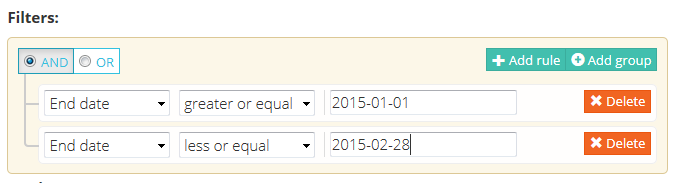
\includegraphics[width=15.24cm,height=4.064cm]{userguide-img/userguide-img006.png}
 
\end{enumerate}

\subsection[edit a view]{edit a view}
\begin{enumerate}
\item Click the \textbf{Data} tab in the top navigation.
\item Click on the \textbf{View} dropdown and select the view you wish to edit. The screen will now be displaying the view you want to edit.
\item Click on the \textbf{View} dropdown again and select \textbf{Edit this view}.
\begin{notebox}
NOTE: If you cannot see the Edit this view option in the View dropdown menu then you do not have permission to edit the view. \ 
\end{notebox}

\item Make any changes you wish to make. You can rename your view, hide or unhide columns, or reset your filter or sort criteria. 
\item To save your changes click the \textbf{Save} button at the bottom of your page. 
\end{enumerate}
\subsection[delete a view]{delete a view}
\begin{enumerate}
\item Click the \textbf{Data} tab in the top navigation.
\item Click on the \textbf{View} dropdown and select the view you wish to delete. The screen will now be displaying the view you want to delete.
\item Click on the \textbf{View} dropdown again and select \textbf{Edit this view}.
\begin{notebox}
NOTE: If you cannot see the Edit this view option in the View dropdown menu then you do not have permission to edit this view. \ 
\end{notebox}

\item Scroll down to the bottom of the screen and click the \textbf{Delete} button.
\item To confirm you want to delete the view, click the \textbf{Delete} button in the pop-up box that appears on your screen. 
\end{enumerate}
\subsection[use the calendar view]{use the calendar view}
If any of your data views include dates you can view these using the calendar view. The calendar view will display each date and date range field on the calendar, with the key for each one shown at the top of the calendar.

\begin{enumerate}
\item Click the \textbf{Data} tab in the top navigation.
\item Click on the \textbf{View} dropdown and select the view you wish to see. 
\item Click on the \textbf{Calendar icon}
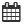
\includegraphics[width=0.635cm,height=0.635cm]{userguide-img/userguide-img007.png}
 at the top of the page. 
\end{enumerate}
\subsection[view data as a graph]{view data as a graph}
\label{subsec:viewgraph}
You can also see data in graph format. Graphs are configured by system administrators. They decide which fields are included in each graph and the form the graph will take (i.e. pie, bar, etc). To see these graphs:

\begin{enumerate}
\item Click on your name at the top of the page.
\item Select \textbf{My graphs} from the dropdown menu.
\item Tick the graphs you would like to be able to see and click \textbf{Save}.
\item \ Next, click the \textbf{Data} tab in the top navigation.
\item Click on the \textbf{View} dropdown and select the data view you wish to display a graph for. 
\item Click on the \textbf{Graph icon}
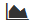
\includegraphics[width=0.9cm,height=0.609cm]{userguide-img/userguide-img008.png}
 at the top of the page. 
\item If this is the first time you are viewing graphs and you have skipped steps 1 to 3 then you will see a link to a page where you can select which of the configured graphs you want to see. Tick all the graphs you would like to see and click the \textbf{Save} button. 
\item You should now see all the available graphs for that view displayed on a single screen. Some of the graphs may be `empty' if your selected data view doesn't include the data fields that the graphs are set up for. 
\begin{notebox}
NOTE: When you click on the Graph icon, all the graphs that you see on that page will only be using the data included in the view you have selected. You can see the data in any global or personal data view in terms of the graphs that have been set up. By setting up a personal view \ you can control exactly what data you want included in a graph. 
\end{notebox}

\item To return to a table view click on the Table icon
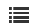
\includegraphics[width=0.926cm,height=0.714cm]{userguide-img/userguide-img009.png}
 
\end{enumerate}
\subsection[hide graphs you don{}'t want displayed]{hide graphs you don't want displayed}
\begin{enumerate}
\item Click on your name at the top of the page.
\item Select \textbf{My graphs} from the dropdown menu.
\item De-select the graphs you no longer want \ to see and click \textbf{Save}.
\end{enumerate}

\clearpage\section[ALERTS: Setting alerts]{ALERTS: Setting alerts}
You can set alerts so that you receive an email notifying you when someone else has updated data you are interested in. The alert will be sent to the email address that you use to log in to the system. 

\subsection[set a change alert ]{set a change alert }
\label{subsec:setalert}
Before you set your change alert, you may need to \hyperref[subsec:personalview]{create a data view} that includes the record(s) and/or fields you want to monitor, if one does not already exist. Any changes to the view will cause an alert to be sent, be it new rows appearing in the view, rows disappearing, or data items changing in fields that are included in the row. Once you have set up and selected your view you need to: 

\begin{enumerate}
\item Click the \textbf{Data} tab in the top navigation.
\item Click on the \textbf{View} dropdown again and select \textbf{Alert me}.
\item In the pop-up box, select whether you want to receive notifications \textbf{Instantly} or \textbf{Every 24 hours}. If you select \textbf{Every 24 hours}, you will receive a daily summary email of all the alerts, normally overnight.
\item Click the \textbf{Save} button. 
\end{enumerate}
\begin{tipbox}[userdefinedwidth=15cm]
    \textbf{Tip:} In any \hyperref[subsec:personalview]{data view} you save, you can select which data fields (columns) you want to include, and you can use \hyperref[subsec:viewstofilter]{filters} to only show records (rows) that meet specific criteria. For example, to set an alert on one specific record you would first need to create a view that only shows that record. 
\end{tipbox}

\subsection[cancel or change an alert ]{cancel or change an alert }
\label{subsec:changealert}
\begin{enumerate}
\item Click the \textbf{Data} tab in the top navigation.
\item Click on the \textbf{View} dropdown again and select \textbf{Alert me}.
\item In the pop-up box, change your alert to \textbf{Instant} or \textbf{Every 24 hours}, or select \textbf{Never} if you want to cancel the alert.
\item Click the \textbf{Save} button. 
\end{enumerate}

\begin{admin}
\clearpage\section[FIELDS: Adding, editing and deleting data fields ]{FIELDS: Adding, editing and deleting data fields }
\subsection[add a new field]{add a new field}
\label{subsec:addfield}
\begin{enumerate}
\item Click the \textbf{Admin} tab in the top navigation and select \textbf{Data Layout} from the drop-down menu. (If you can't see the \textbf{Admin} tab, then you don't have the permissions to add, edit or delete data fields.)
\item Click on the \textbf{Create new field} button. 
\item You will be presented with the \textbf{Create new field} screen.
\item Give your field a name e.g. Project. (You can use spaces and special characters in field names.) 
\item Select the \textbf{Type} of field from the dropdown list

\begin{enumerate}
\item Text -- Lets users enter single words and strings of words and number
\item Integers -- Lets users enter whole numbers only, no letters or symbols
\item Date -- Lets users select a date
\item Date range -- Lets users select a start and an end date
\item Dropdown list -- Lets you provide multiple options for users to choose from

\begin{itemize}
    \item When you select this field type click the \textbf{Add} button on the right-hand side of the screen for each option you want to add.
\item Click on the x next to the box to delete an item. 
\end{itemize}
\item Tree \ {}-- Rather than confusing users with a long list of items to choose from, using a tree to structure the options makes it easier for them to find the item they need. See: \hyperref[subsec:fieldtree]{Use a tree to structure categories and sub-categories}
\item Document {}-- Lets users upload a document
\item Person {}-- Lets users select from a list of all other users on the system.
\item RedAmberGreen status (RAG) \--- Automatically generates colour-coded indicators based on the values of other data fields. See: \hyperref[subsec:fieldrag]{Add a status indicator to a record}
\item Calculated value {}-- Lets you automatically generate values based on other fields. See: \hyperref[subsec:fieldcalc]{Automatically calculate values for a field}
\item Record from other data sheet -- Lets you provide multiple options for users to choose from, which are populated from another data sheet.

\begin{itemize}
    \item When you select this field type select the other data sheet from the right-hand side of the screen.
    \item Tick the columns you wish to the user when displaying the options.
\end{itemize}
\end{enumerate}
\item Once you have selected the field type and completed the relevant options for that field you can add a \textbf{Description} which all users will see displayed next to the field. 
\item You can also add \textbf{User help text}. This is displayed when a user clicks on the question mark (?) next to the field name. 
\item Tick the box if you want the field to be optional.
\item Click \textbf{Save} to create the new data field. 
\item Under \textbf{Permissions} set which user groups can view and edit this data field by clicking on the \textbf{Add new group} button. You must \hyperref[sec:usergroups]{add at least one user group} here, otherwise the field will be invisible to all users. For more information see \hyperref[subsec:setfieldperms]{Set permissions for data fields}.
\end{enumerate}

\subsection[set permissions on a data field]{set permissions on a data field}
\label{subsec:setfieldperms}
By using the Linkspace groups functionality, you can set who can view, add, edit or approve changes to specific data fields according to the user group(s) they belong to. For each data field you can specify what members of each user group are allowed to do on that field.

To set permissions on a data field, there are two steps:

\textbf{The first step is to set up your groups.}

\begin{enumerate}
    \item Click the \textbf{Admin} tab in the top navigation.
    \item Select \textbf{Manage Groups} from the dropdown menu.
    \item Click the \textbf{Create new group} button.
    \item Give the group a name and click \textbf{Save}.

\begin{notebox}
NOTE: When you set up a new user you should allocate them to one of the groups you have created. If they are not allocated to a group, they will not be able to see or edit any data fields on which you have set group permissions.
\end{notebox}

\textbf{Then you need to set the groups’ permissions on the data field.}

    \item \hyperref[subsec:addfield]{Add a new data field}.
    \item Under \textbf{Permissions} on the data field screen, click \textbf{Add new group}.
    \item For each new group you can select what users of that group can do on that field i.e. Read values; Enter values for new records; Edit values of existing records; Approve values in new records; Approve changes in existing records; Enter values for new records without requiring approval; Edit values of existing records without requiring approval.
    \item Click \textbf{Save}.

\begin{notebox}
NOTE: If you do not define the permissions for a group on a data field then it will automatically hide that field from everyone in that group. 
\end{notebox}

\end{enumerate}

\subsection[control when a field is displayed]{control when a field is displayed}
You can choose to hide or display a field on the New record or Edit record screen according to the value of another field. \ This can make your New/Edit record screen less overwhelming, by only showing fields that are directly relevant. 

To do this, tick the box next to \textbf{Only display under the following conditions} when you are \hyperref[subsec:addfield]{adding a new field}. In the first box, select the field on which your condition is based. In the second box, enter the required text of an exact match, or use a Regular Expression for any other type of match. For example:

\begin{flushleft}
\tablefirsthead{}
\tablehead{}
\tabletail{}
\tablelasttail{}
\begin{supertabular}{|m{8.048cm}|m{6.1590004cm}|}
\hline
For an exact match  &
Enter the text you want to match\\\hline
To match any non-blank value &
.+\\\hline
To match any of three values e.g. {\textquotedbl}val1{\textquotedbl}, {\textquotedbl}val2{\textquotedbl} or {\textquotedbl}val3 (comment){\textquotedbl}:

~
 &
(val1{\textbar}val2{\textbar}val3 {\textbackslash}(comment{\textbackslash}))

~
\\\hline
To match a value containing the word {\textquotedbl}foo{\textquotedbl} &
.*foo.*\\\hline
To match anything beginning with {\textquotedbl}bar{\textquotedbl} &
bar.*\\\hline
To match any number &
[0-9]+\\\hline
\end{supertabular}
\end{flushleft}
\subsection[automatically calculate values for a field]{automatically calculate values for a field}
\label{subsec:fieldcalc}
You can create a \textbf{Calculated value} data field to automatically generate values based on other fields. 

\begin{enumerate}
\item \hyperref[subsec:addfield]{Add a new data field} and give it a name. 
\item Select \textbf{Calculated value} as the \textbf{Type} of field. 
\item In the \textbf{Return value conversion} dropdown box, select whether the final value will be text, a date, a number or an integer.
\item In the \textbf{Calculation} box, use the Basic Perl programming style to return the value of the calculated field. To reference another field insert the field name in square brackets and the value(s) of the field in inverted commas. For example if you wanted to create an automatically generated Continent field that depended on the value in the Country field, you might use the following:

\begin{code}
if ([Country] eq "Greece") {
    return "Europe"
} elsif ([Country] eq "Japan") {
    return "Asia"
}
\end{code}

You can also reference the ID of the record instead of a specific field by using id. For example

\begin{code}
if ([id] < 20) {
    return "Early phase project"
} else {
    return "Phase 1 project"
}
\end{code}

If you wanted two or more criteria to apply for a specific value to be returned in your Continent field you might use the following:

\begin{code}
if ([Country] eq "Greece" && [Region] eq "A") {
    return "Out of area"
}
\end{code}

You can set criteria on values in date ranges by adding the suffix {\textquotedbl}.from{\textquotedbl} or {\textquotedbl}.to{\textquotedbl} to the field. For example, if you had a planning phase (field name: "Planning phase") on every project, and you wanted to show which projects were currently doing their planning (i.e. where today's date falls within that date range) you might use the following:

\begin{code}
if ([Planning phase.from] > CURDATE) {
    return "Started"
}
\end{code}

Or, if you wanted to return a value for the calculated field based on it being greater than or less than the amount specified in the data field named Cost, you might use: 

\begin{code}
if ([Cost] < 10) {
    return "Bargain"
}
\end{code}

You can also return a value based on the sub-category of a tree. For example: you have a field called Countries, which you set up as a tree listing all the countries under each continent.

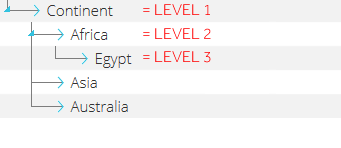
\includegraphics[width=6.692cm,height=2.903cm]{userguide-img/userguide-img010.png}
 

In this example, all the continents would be level 2 nodes in the tree, and all the countries would be level 3 nodes. If you wanted to return a value based on the continent, rather than the country that had been selected you could specify this by referring to the value at level2. \ 

\begin{code}
if ([Countries.level2] eq "Africa") {
    return "Zone B"
}
\end{code}

\item Click \textbf{Save} to create the new data field. 
\end{enumerate}
\subsection[use a tree to structure categories and sub{}-categories]{use a tree to structure categories and sub-categories}
\label{subsec:fieldtree}
If you have a number of categories and sub-categories that you want users to choose from in a data field, setting it up as a data tree makes it easier for people to find what they're looking for, and eliminates spelling errors. 

\begin{enumerate}
\item \hyperref[subsec:addfield]{Add a new data field} and give it a name.
\item Select \textbf{Tree} as the \textbf{Type} of field. 
\item Tick the \textbf{Only all end-nodes to be selected} if you want users to be able only to select the final sub-categories in the tree and not higher-level categories.
\item Each item in the tree is referred to as a node. Similar to a folder structure on your computer, you create top-level nodes and can then nest other nodes underneath these. To start click the \textbf{Create} button under the \textbf{Node selection} box. 
\item To add a node underneath another node, select the node you want as the parent and click \textbf{Create} again.
\item To rename or delete a node, select it and click on either the \textbf{Rename} or \textbf{Delete} button. 
\item Set the permissions for the field and click \textbf{Save} to create the new data field. 
\end{enumerate}
\subsection[add a status indicator to a record ]{add a status indicator to a record }
\label{subsec:fieldrag}
You can create a \textbf{RedAmberGreen indicator field} to automatically generate colour-coded indicators based on other fields. The conditions for the red, amber and green indicators will always be checked in that order. If a record meets more than one of the conditions, it will show the red over the amber or the green. 

\begin{enumerate}
\item \hyperref[subsec:addfield]{Add a new data field} and give it a name.
\item Select \textbf{RedAmberGreen (RAG) status} as the \textbf{Type} of field. 
\item Use Basic Perl programming style to stipulate the conditions for red, amber and green indicators to be displayed. If none of the conditions match, the field will be grey. \newline
Values from other fields are used by inserting the field name between square brackets, whilst {\textquotedbl}CURDATE{\textquotedbl} can be used to insert the current date. \newline
For example, if you wanted a green indicator for projects where the start date was in the past you might use: 
\begin{code}
[Start Date] {\textless} CURDATE\newline
\end{code}

Or if you wanted a red alert where a project was over budget you might use: \newline

\begin{code}
[Cost to date] > [Budget]
\end{code}

\item Set the permissions for the field and click \textbf{Save} to create the new data field. 
\end{enumerate}
\subsection[change the order of the fields]{change the order of the fields}
Any changes you make to the order of the fields will affect all your users. 

\begin{enumerate}
\item Click the \textbf{Admin} tab in the top navigation and select \textbf{Data Layout} from the drop-down menu. (If you can't see the \textbf{Admin} tab, then you don't have the permissions to add, edit or delete data fields.)
\item Drag and drop the fields to reorder them. 
\item When you are finished click \textbf{Save order}.
\end{enumerate}
\subsection[edit a field]{edit a field}
\begin{enumerate}
\item Click the \textbf{Admin} tab in the top navigation and select \textbf{Data Layout} from the drop-down menu. (If you can't see the \textbf{Admin} tab, then you don't have the permissions to add, edit or delete data fields.)
\item Click the \textbf{Edit} link next to the name for \ the field you want to change.
\item Make your changes and click \textbf{Save}.
\end{enumerate}

\bigskip

\subsection[delete a field]{delete a field}
\begin{enumerate}
\item Click the \textbf{Admin} tab in the top navigation and select \textbf{Data Layout} from the drop-down menu. (If you can't see the \textbf{Admin} tab, then you don't have the permissions to add, edit or delete data fields.)
\item Click the \textbf{Edit} link next to the name for the field you want to change.
\item Scroll down to the bottom of the Edit data field screen and click the \textbf{Delete button}.
\item To confirm you want to delete the field, click the \textbf{Delete} button in the pop-up box that appears on your screen. \textbf{IMPORTANT: Once you delete a field you will lose all the data stored in that field}. 
\end{enumerate}

\clearpage\section[PERMISSIONS: Seting permissions]{PERMISSIONS: Setting permissions}
Linkspace enables very fine control over exactly what data users can add, delete, view and update. You control what users are able to do and see on the Linkspace system in two ways:
\begin{enumerate}
    \item You control what data fields they can view, edit and approve changes on via their membership of user groups – See: \hyperref[subsec:setfieldperms]{Set permissions on a data field}.
    \item You control everything else they can do on the system (i.e delete records, download data, manage user accounts, administer layouts, views and graphs, etc. via their individual user permissions – See: \hyperref[subsec:userperms]{Set the permissions for a user}).
\end{enumerate}

\clearpage\section[USER GROUPS]{USER GROUPS}
\label{sec:usergroups}

\subsection[set up a new user group]{set up a new user group}
\begin{enumerate}
    \item Click the \textbf{Admin} tab in the top navigation.
    \item Select \textbf{Manage Groups} from the dropdown menu.
    \item Click the \textbf{Create new group} button
    \item Give the group a name and click \textbf{Save}.
\end{enumerate}
\begin{notebox}
NOTE: There are no system-wide field permissions associated with groups. You need to specify the permissions that each group has for each data field. You can see an overview of a group’s permissions across all fields by going to Admin > Manage Groups
\end{notebox}

\subsection[delete a user group]{delete a user group}
\begin{enumerate}
    \item Click the \textbf{Admin} tab in the top navigation.
    \item Select \textbf{Manage Groups} from the dropdown menu.
    \item Click the \textbf{Edit name} link next to the group you want to delete.
    \item Click the \textbf{Delete} button and then \textbf{Confirm deletion} on the pop up box.
\end{enumerate}

\clearpage\section[GRAPHS: Set up]{GRAPHS: Set up}
\subsection[create a new graph ]{create a new graph }
Only users with permission to configure the system itself can create graphs. Other users can control the data that is included in the graphs through creating personalised views of the data. See: \hyperref[subsec:viewgraph]{View data as a graph}

\begin{enumerate}
\item Click the \textbf{Admin} tab in the top navigation and select \textbf{Graphs} from the drop-down menu. (If you can't see the \textbf{Admin} tab, then you don't have the permissions to add, edit or delete data fields or graphs.)
\item Click on \textbf{Create new graph}.
\item Provide a title and a description of your graph. 
\item Select the \textbf{Type} of graph: Bar, Line, Donut, Scatter or Pie
\item Define the data fields and values for your graph. 
\item Select a field for the \textbf{X-axis} from the dropdown list. This defines the set of values to use for the x-axis (horizontal axis) for a bar, line or scatter graph. For a donut or pie graph, this defines each segment within a ring. The x-axis label will automatically be the name of its defined data field. It's also possible to select all <All fields in view>, which will show each field in the view as a point on the x-axis. This option is only really applicable when summing fields (see below); a count will produce a flat graph across all points.
\item The \textbf{X-axis grouping} is optional and only relevant to date fields. It lets you group the values that are returned for the x-axis according to day, month or year. 
\item From the dropdown list, select the field to use for your \textbf{Y-axis field}. This defines the field to use for the y-values (vertical axis) of a graph. You can ignore this step if you are using a donut or pie graph, or if you want your y-axis to show a total count for each value that appears in the X-axis field. \ 
\item In the \textbf{Y-axis values} box you must choose whether you want the graph to show the total sum of a particular field (for numeric values only), or count the number of times each value appears. 
\item If you are using a bar, line or scatter graph, provide a \textbf{Y-axis label}.
\item The \textbf{Group by field} is optional. This lets you group related data items. For example, if countries were being displayed on the graph, this option could be used to group (and colour code) by continent. In the case of a donut graph, this defines the rings. Otherwise, the data being displayed is normally a smaller subset of this grouping option.
\item Select a set of metrics if you want your values to be converted to percentage values compared against a set of fixed values. See the \hyperref[sec:metrics]{metrics} section for more information.
\item Select \textbf{Stack data} if you want different data items for the same x value to be stacked on top of each other, rather than displayed side-by-side
\item Select \textbf{Add graph to all users} if you want the graph to be displayed in the graph view for all users.
\item Click the \textbf{Save} button at the bottom of the screen.
\end{enumerate}
\subsection[edit a graph ]{edit a graph }
\begin{enumerate}
\item Click the \textbf{Admin} tab in the top navigation and select \textbf{Graphs} from the drop-down menu. (If you can't see the \textbf{Admin} tab, then you don't have the permissions to edit graphs.)
\item Click on the \textbf{Edit} link next to the graph you wish to edit. 
\item Make any changes and click the \textbf{Save} button at the bottom of the screen.
\end{enumerate}
\subsection[delete a graph ]{delete a graph }
\begin{enumerate}
\item Click the \textbf{Admin} tab in the top navigation and select \textbf{Graphs} from the drop-down menu. (If you can't see the \textbf{Admin} tab, then you do not have the permissions to edit graphs.)
\item Click on the \textbf{Edit} link next to graph you wish to edit.
\item Click the \textbf{Delete} button at the bottom of the screen.
\item To confirm you want to delete the graph, click the \textbf{Delete} button in the pop-up box that appears on your screen. 
\end{enumerate}


\clearpage\section[METRICS: Compare graphs against absolute values]{METRICS: Compare graphs against absolute values}
\label{sec:metrics}
Metrics enable a graph's values to be converted into percentage values, measured against pre-defined values. For example, a graph might have y-axis values of 20, 40 and 50. These could be plotted against metrics of 40, 40 and 200 (which might be targets). In this case, the graph values would be converted to 50\%, 100\% and 25\%.

\subsection[create a set of metrics]{create a set of metrics}
One set of metrics consists of several points to plot a graph against. Only users with permission to configure graphs can create metrics.

\begin{enumerate}
\item Click the \textbf{Admin} tab in the top navigation and select \textbf{Metrics} from the drop-down menu. (If you can't see the \textbf{Admin} tab, then you don't have the permissions to add, edit or delete data fields or graphs.)
\item Click on \textbf{Create new metric}.
\item Provide a name for the metrics.
\item Click \textbf{Create}.
\end{enumerate}
\subsection[add data points to a metric set]{add data points to a metric set}
\begin{enumerate}
\item Click \textbf{Edit} next to the name of the relevant metric set.
\item To add a metric point, click \textbf{Add Item}.
\item To edit an existing metric point, click \textbf{Edit} next to the item.
\item For each metric point, enter the x-axis value that the metric applies to. The value must be exactly how it is shown on the graph. Also enter the y-axis value that the graph's value should be ccompared against. Optionally, enter a y-axis grouping value, if the graph in question has a y-axis grouping set (thereby having more than one value per x/y coordinate).
\item Click the \textbf{Save} button.
\end{enumerate}

\subsection[delete a metric group]{delete a metric group}
\begin{enumerate}
\item Click \textbf{Edit} next to the name of the relevant metric set.
\item Click \textbf{Delete group}.
\end{enumerate}

\subsection[remove a data point from a metric set]{remove a data point from a metric set}
\begin{enumerate}
\item Click \textbf{Edit} next to the name of the relevant metric set.
\item Click \textbf{Edit} next to the item.
\item Click \textbf{Delete}.
\end{enumerate}


\clearpage\section[MESSAGES: Emailing other users]{MESSAGES: Emailing other users}
\subsection[email another user from linkspace]{email another user from linkspace}
If the names of other users are included in your data records as a person field, you can access their email address by clicking on their name in the record. If you have an email client installed on your device you can then click on the email address to create a new email message addressed to that user. \ 

\subsection[email a group of users]{email a group of users}
Linkspace makes it easy to message a group of users that appear in a person field. For example, if your record has a person field called Project leaders, you can email all the project leaders simply by clicking on the envelope icon at the top of the Project leaders column.

What makes it more powerful is that you can filter the list according to certain criteria and then use the same action to message all project leaders whose projects meet those criteria. 

For example, if you wanted to email all of the project leaders whose projects had budgets over {\pounds}10,000, you would \hyperref[subsec:viewstofilter]{use a filter} to view only those projects where [Budget] greater 10000. In that view you can then click on the envelope icon at the top of the Project leaders column to email the leaders of only those projects. 


\end{admin}

\clearpage\section[LOGIN: Managing your account details]{LOGIN: Managing your account details}
\subsection[change your password]{change your password}
Linkspace does not allow you to set your own password, but you can ask the system to generate a new one for you. If you are already logged in:

\begin{enumerate}
\item Click on \textbf{your name} at the top of the screen
\item Select \textbf{My details} from the dropdown menu
\item Click on the \textbf{Change password} button at the bottom of the screen. 
\item Enter your current password in the text box on the pop-up screen and click on the \textbf{Generate new password} button.
\item Your new password will be displayed on the screen. 
\end{enumerate}
\subsection[request a new password]{request a new password}
If you have forgotten your password

\begin{enumerate}
\item Click on the \textbf{Reset password} link on the login page
\item Enter your email in the text box in the pop up screen.
\item Click \textbf{Submit}
\item You will be emailed a link to reset your password. 
\end{enumerate}
\subsection[edit your personal details]{edit your personal details}
\begin{enumerate}
\item Click on \textbf{your name} at the top of the screen
\item Select \textbf{My details} from the dropdown menu
\item Make you changes and click on the \textbf{Save} button at the bottom of the screen. 
\end{enumerate}
\begin{notebox}
NOTE: If you change your email address this will become your new username when you log in. 
\end{notebox}

\begin{admin}
\clearpage\section[USERS: Managing users ]{USERS: Managing users }
\subsection[add a new user to the system ]{add a new user to the system }
\begin{enumerate}
\item Click the \textbf{Admin} tab in the top navigation and select \textbf{Manage Users} from the drop-down menu. (If you can't see the \textbf{Admin} tab, then you don't have the permissions to add, edit or delete users.)
\item Click on \textbf{Create user}.
\item Complete the new user form and click \textbf{Save}.
\end{enumerate}
\begin{tipbox}[userdefinedwidth=15cm]
\textbf{Tip:} It is possible for Linkspace users to request an account through your Linkspace login screen. If this functionality is enabled on the system, direct users to your login URL. You will be alerted to any new account requests. \
\end{tipbox}

\bigskip

\subsection[set the permissions for a user]{set the permissions for a user}
\label{subsec:userperms}
You can set permissions for each user on the system. If a user has no permissions they can only view data, and add and remove the graphs displayed on their personal page. To set user permissions:
\begin{enumerate}
    \item Click the \textbf{Admin} tab in the top navigation and select \textbf{Manage users}.
    \item Click on the \textbf{ID number} of the user you wish to edit.
    \item Use the tick boxes under the Permissions section to set what the user is able to do.
    \item Click \textbf{Save}.
\end{enumerate}

\begin{notebox}
    NOTE: Permissions explained
\end{notebox}

\begin{flushleft}
\tablefirsthead{}
\tablehead{}
\tabletail{}
\tablelasttail{}
\begin{supertabular}{|m{3.046cm}|m{10.915cm}|}
\hline
User can delete records &
This permission allows a user to permanently delete records, including their version history \ \\\hline
User can manage other user accounts &
This permission allows a user to manage user accounts on the system, including the configuration of permissions \\\hline
User can download data &
This permission allows a user to download data in CSV format \\\hline
User can administer layout, views and graphs &
This permission allows a user to configure the system itself, including the configuration of the layout and graphs, and the creation of global views \\\hline
User can send messages &
This permission allows a user to send messages to users, using the messaging capability in the tabular data view \ \\\hline
User can create, modify and delete views &
This allows a user to create, modify or delete views. Unless the user has the administer layout permission, the views can only be personal views. \ \\\hline
\end{supertabular}
\end{flushleft}

\subsection[approve a new user ]{approve a new user }
If you are an administrator responsible for approving new users you will receive an email alert when a new user requests a user account. To approve the request:

\begin{enumerate}
    \item Click the \textbf{Admin} tab in the top navigation and select \textbf{Manage Users} from the drop-down menu. (If you can't see the \textbf{Admin} tab, then you do not have the permissions to add, edit or delete users.)
\item New Account requests are displayed below the list of Active accounts.
\item Click on the \textbf{ID} of the user you wish to approve.
\item Click \textbf{Approve} to activate the account.
\end{enumerate}
\subsection[edit user details]{edit user details}
\begin{enumerate}
\item Click the \textbf{Admin} tab in the top navigation and select \textbf{Manage Users} from the drop-down menu. (If you can't see the \textbf{Admin} tab, then you don't have the permissions to add, edit or delete users.)
\item Click on the \textbf{ID} of the user you wish to edit.
\item Change the details as required and click \textbf{Save}.
\end{enumerate}
\clearpage\section[APPROVAL: Approving changes]{APPROVAL: Approving changes}
If there are any new records or edits that require approval any user with the authority to approve changes will be able to see this immediately when they login. The number of records requiring approval will be shown in brackets next to the Approval tab in the top navigation. 

\subsection[approve a change]{approve a change}
\begin{enumerate}
\item Click the \textbf{Approval} tab in the top navigation. (If you can't see the \textbf{Approval} tab, then you do not have the permissions to approve changes or new records.)
\item You will see a list of all the records requiring approval. 
\item Click on the record \textbf{ID} to view the record you want to check. If it is a new record, all fields will be displayed on the following screen. If it is a changed record, only the fields that need approval will be displayed. 
\item Once you are happy with the changes, click the Approve button at the bottom of the page. 
\end{enumerate}

\end{admin}

\clearpage\section{SEARCH: Searching for data}

\subsection[use the wildcard search]{use the wildcard search}
You can use the search box at the top of the screen to find specific records. If you want to search across all fields but are not sure of the exact spelling or full term used, you can use the wildcard function. \ Use the * to indicate that what you've typed is only a part of what you are looking for.

For example, if you wanted to find a specific project, but didn't know the full project name, you could type the part you do know inside two *s -- i.e. *Training*. The search will return all records where there is a reference to training in the project name, or in any other field. Results will be shown in accordance with the current view (with the filter removed, showing the results of the search instead).

\begin{notebox}
NOTE: The search can be run faster when you search using the beginning of something i.e. only using the * at the end. For example if you wanted to search for all countries that start with United, you would type United* in the search box. 
\end{notebox}

\begin{admin}
\clearpage\section[Linkspace HOMEPAGE]{Linkspace HOMEPAGE}
\subsection[configuring your linkspace homepage]{configuring your linkspace homepage}
You can add text and links to your Linkspace homepage.

\begin{enumerate}
\item Click the \textbf{Admin} tab in the top navigation and select \textbf{General Settings} from the drop-down menu. (If you can't see the \textbf{Admin} tab, then you don't have the permissions to add, edit or delete users.)
\item Use the WYSIWIG editor to add and format any text you want to add to your system's home page.
\item Click \textbf{Save}.
\end{enumerate}
\end{admin}

\end{document}
